\documentclass[12pt, a4paper]{article}

\usepackage[czech]{babel}
\usepackage[IL2]{fontenc}
\usepackage[utf8]{inputenc}
\usepackage{lmodern}  % lepší kvalita PDF

\usepackage[a4paper,top=3cm,bottom=3cm,left=3cm,right=3cm,marginparwidth=1.75cm]{geometry}

\usepackage{graphicx}
\usepackage{titling}
\usepackage{enumitem}
\usepackage{caption}
\usepackage{float}
\usepackage{pdfpages}
\usepackage{verbatim}
\usepackage{amsmath}

\usepackage{listings}
\lstset{numbers=left,
	inputencoding=latin1,
	basicstyle=\scriptsize\ttfamily,
	keywordstyle=\color{blue},
	breaklines=true, 
	showtabs=false,
	showstringspaces=false,
	numberstyle=\tiny\color{gray},
}

\usepackage{multirow}

\usepackage{pkg-custom-commands}
\usepackage{pkg-url}


% údaje na titulní straně
\title{Samostatná práce}
\def \thesubtitle {KIV/VSS}
\author{Patrik Harag}
\def \theauthoremail {harag@students.zcu.cz}
\def \theauthorid {A18N0084P}

\begin{document}

\begin{titlepage}
	\begin{figure}
		
\includegraphics[height=50mm]{img-fav-logo}
	\end{figure}
	
	\centering
	{\large \hspace{1mm} \par} % tady musí být nějaký text jinak nefunguje vertikální odsazení
	\vspace{15ex}
	
	{\huge\bfseries \thetitle \par}
	\vspace{2ex}
	{\scshape\Large \thesubtitle \par}
	\vspace{15ex}
	{\Large\itshape \theauthor \par}
	\vspace{2ex}
	{\texttt{\theauthoremail} \par}
	\vspace{1ex}
	{\texttt{\theauthorid} \par}
	
	\vfill

	{\today\par}
\end{titlepage}


\section*{Zadání}
Simulace šíření vody v krajině na bázi celulárního automatu.


\section*{Analýza}
Zadání bylo úmyslně zvoleno velmi volné, protože bylo nejprve potřeba promyslet podobu simulace.
Zvažováno bylo několik možností:
\begin{itemize}
	\item 2D simulace -- \uv{ze strany}, typu \uv{falling sand} (např. jako \footnote{\url{https://github.com/Hartrik/Sand-Game-2}}), případně i včetně simulace tlaku vody,
	\item pseudo 3D simulace -- simulovat \uv{sloupce} vody na výškové mapě,
	\item 3D simulace -- simulovat \uv{kostičky} vody v \uv{kostičkovém} terénu.
\end{itemize}
Nakonec byla zvolena druhá možnost, tedy simulovat šíření vody na výškové mapě.
Simulace je oproti třetí možnosti zjednodušena v tom smyslu, že v terénu nemohou vznikat převisy, tunely apod.
Voda bude reprezentována jako množství na dané pozici a~nemůže tak být simulováno její padání nebo déšť.

\paragraph{Návrh simulace}
Simulace bude mít jednoduchá pravidla.
V jednom kroku budou navštíveny všechny pozice.
Pro každou pozici bude nalezena sousední pozice s~největším rozdílem \emph{výška + úroveň vody} a dojde k přesunutí až poloviny vody.
Jako okolí může být použito například Moorovo okolí.

\paragraph{Způsob procházení}
Přepočítávání množství vody na jednotlivých pozicích ne\-může být prováděno v systematickém pořadí, protože jinak by docházelo k ubýhání vody k určitému směru.
Z tohoto důvodu musí být pozice procházeny náhodně.


\section*{Implementace}
Pro implementaci byl zvolen programovací jazyk Java a framework JavaFX.
Program má následující strukturu:
\begin{itemize}
	\item \code{cz.harag.vss.sp} -- Obecné doménové třídy, hlavní logika.
	\item \code{cz.harag.vss.sp.render} -- Třídy týkající se renderování výškové mapy, gradienty.
	\item \code{cz.harag.vss.sp.ui} -- Uživatelské rozhraní a 3D vizualizace.
\end{itemize}

\section*{Obsluha}

\paragraph{Kompilace a spuštění}
Program se zkompiluje spuštěním \code{build.bat} (je nutné mít nainstalovaný gradle) a spustí spuštěním \code{run.bat} (vyžaduje Javu 8).
Program lze také spustit s cestou k souboru s terénem jako parametrem.

\paragraph{Terén}
Terén je definován jako obrázek ve formátu PNG.
Výšku udává první bajt (červená složka obrázku).
Několik ukázkových terénů je přiloženo.

\begin{figure}
	\centering
	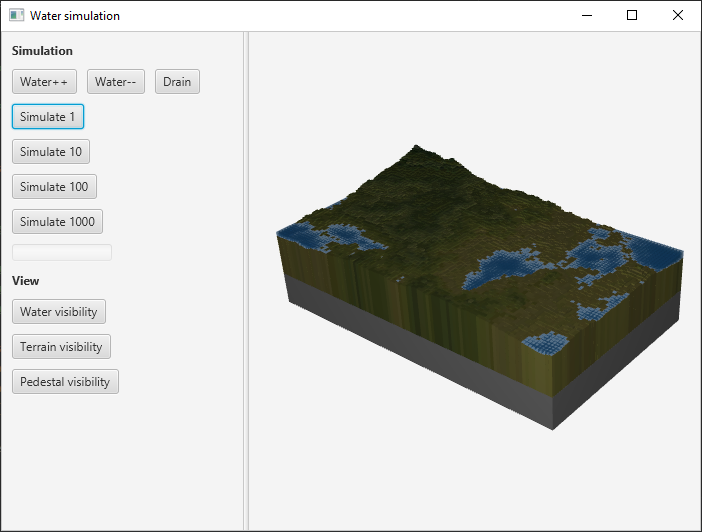
\includegraphics[width=0.9\linewidth]{gui}
	\caption{Hlavní okno aplikace}
	\label{fig:gui}
\end{figure}

\paragraph{Ovládání}
Při nezadání parametru program začne volbou terénu.
Poté je zobrazeno hlavní okno aplikace, viz Obrázek \ref{fig:gui}.
Zde je možné přidat vodu a provést \emph{n}~kroků simulace z vybraných možností.
Držením levého tlačítka myši je možné terén otáčet a pravým tlačítkem přibližovat nebo oddalovat.
Je možné vypnout a zapnout viditelnost částí modelu -- vody, terénu a podstavce.
Dále lze upravit poměr v jakém se odvádí voda z jedné pozice do druhé (výchozí je 0.5 -- zprůměrování).

\section*{Závěr}
Byla vytvořena simulace, která na základě velmi jednoduchých pravidel simuluje šíření vody v terénu.
Součástí je i 3D vizualizace.
Pro simulaci může být jednoduše použit vlastní terén.

Výsledky vypadají s přihlédnutím na úroveň detailů simulace poměrně realisticky.
Od animace bylo upuštěno, protože vykreslování scény trvalo příliš dlouho.
Sestavení 3D scény by mohlo být efektivnější -- pro každé políčko je použit jeden kvádr, což má za následek horší výkon u větších terénů.
Na druhou stranu efektivnější řešení založené na vlastní síti polygonů by bylo mnohonásobně náročnější na vytvoření.
Program by mohl být dále vylepšen například umožněním přímým zásahům do terénu -- modifikace terénu, přidání vody na určité místo apod.


% \bibliographystyle{plain}
% \bibliography{references}

% \chapter*{Přílohy}
% \section*{xxx}
% \lstinputlisting[label={xx}, caption={yy}]{sources.java}

\end{document}